% 核心逻辑：World Model 和 test-time-Agent 之间的比较。
% 1. 问题背景：Agent 在 Validation Set 上容易过拟合 (Public LB vs Private LB)。
% 2. 实验设定：计算 Agent Self-Eval 的准确率 (0.72) vs World Model（0.615）。计算World Model在这些 Agent 出错样本上的表现。
% 3. 结论：World Model 作为一个独立裁判，具有更强的泛化稳健性。


\section{Agent Integration: \ours}
\label{sec:agent}

Building on the predictive capabilities of the World Model, we propose \textbf{\ours}, a hybrid autonomous ML agent designed to decouple hypothesis exploration from physical execution. 


\subsection{Motivation}
\label{sec:agent_motivation}

We aim to break the \textit{Execution Bottleneck} in Section~\ref{sec:motivation}, compressing hours of physical execution into seconds of logical inference, and the \textit{Validation-Test Gap} identified in Section~\ref{subsec:rq4_cases}.
Thus, we propose \textbf{\ours}, which utilizes the ``Implicit World Model'' as a filter to prune the search space before execution for acceleration.


\subsection{Method: The Predict-then-Verify Loop}
\label{sec:method}

We adopt \textbf{AIDE}~\cite{jiang2025aideaidrivenexplorationspace} as our backbone, building directly upon the tree-search architecture described in Section~\ref{sec:agent_paradigm}.

We propose \textbf{\ours}, which re-engineers the Improvement stage into a conservative \textit{Predict-then-Verify} loop (Figure~\ref{fig:main}(e)) to bridge the Implementation Gap~\cite{zhu2025aiscientistsfailstrong}.
The workflow proceeds through three key phases: (1) \textbf{High-Volume Generation}, where $m=10$ candidates are proposed in parallel to expand search width without execution costs; (2) \textbf{Confidence-Gated Pairwise Selection}, which utilizes a confidence gate ($c=0.7$) to ensure high-certainty selection; and (3) \textbf{Verification Execution}, where the Top-$k$ ($k=1$) candidate is physically verified to anchor the solution trajectory in execution feedback (see ablation study in Appendix~\ref{app:ablation_k}).

\begin{figure*}[t]
    \centering
    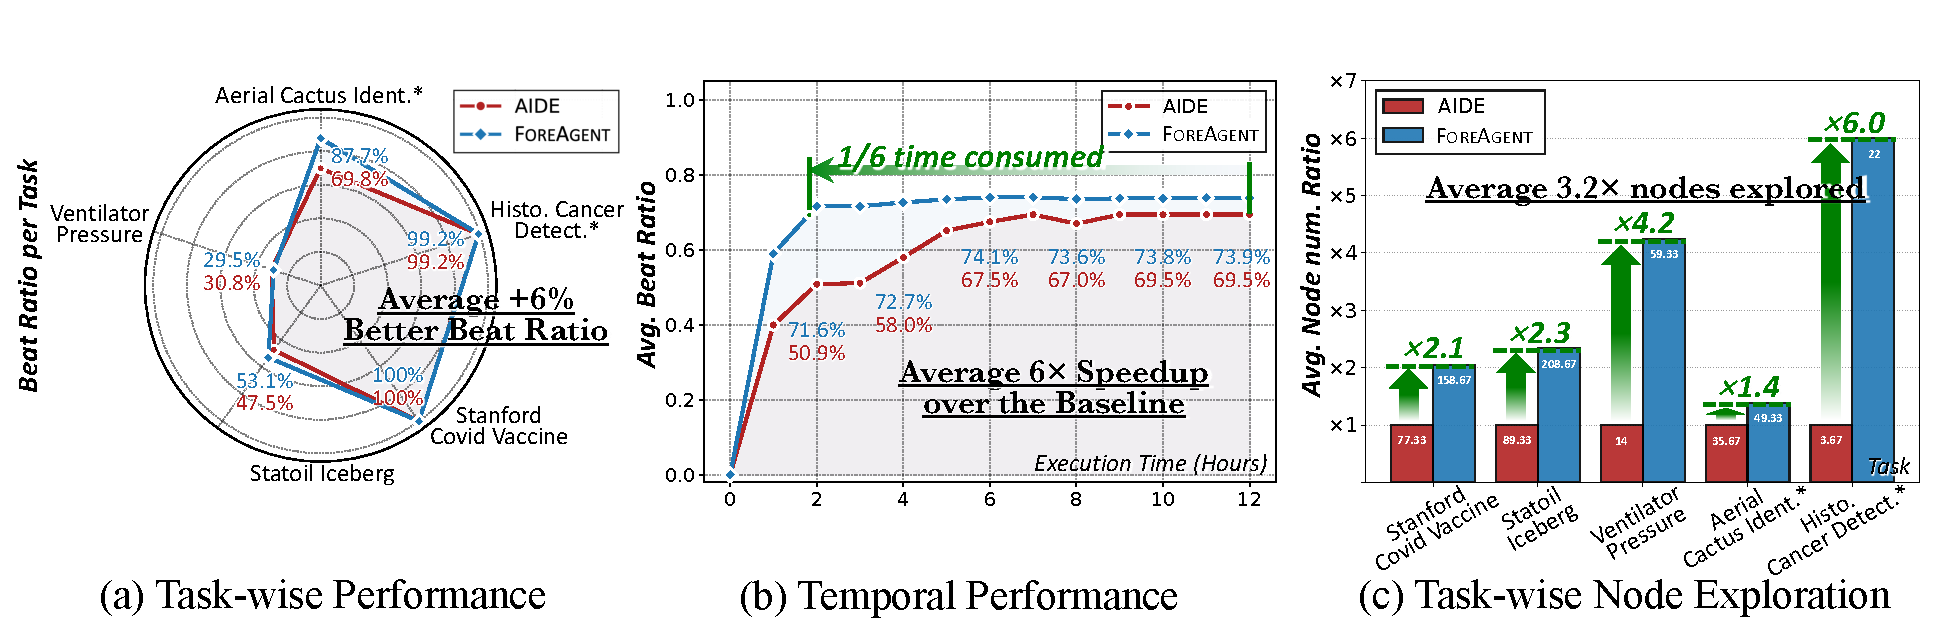
\includegraphics[width=\linewidth]{figures/agent.pdf} % 暂时注释掉真图
    \caption{\textbf{Agent Performance Analysis.}
  (a) \textbf{Task-wise Beat Ratio:} \ours achieves an average +6\% improvement over the AIDE baseline.
  (b) \textbf{Temporal Efficiency:} The agent converges to peak performance using only 1/6 of the execution time, achieving an average $6\times$ speedup.
  (c) \textbf{Search Breadth:} By offloading evaluation to the ``Implicit World Model'', \ours explores $3.2\times$ more nodes on average compared to the baseline, significantly expanding the search space within the same time budget.}
  \label{fig:agent_performance}
\end{figure*}

\begin{table}[h]
\centering
\small
\begin{tabular}{lll}
\toprule
\textbf{Task Name} & \textbf{Domain} & \textbf{Status} \\
\midrule
Stanford Covid Vaccine & Biology & Seen \\
Ventilator Pressure & Physics & Seen \\
Statoil Iceberg & Geoscience & Seen \\
Aerial Cactus Ident.* & Ecology & \textbf{Unseen} \\
Histo. Cancer Detect.* & Medicine & \textbf{Unseen} \\
\bottomrule
\end{tabular}
\vspace{-2pt}
\caption{\textbf{Agent Evaluation Benchmark.} The selection covers diverse AI4Science domains to test the World Model's capability to generalize from seen tasks to unseen scientific problems.}
\label{tab:agent_tasks}
\vspace{-10pt}
\end{table}


\subsection{Experimental Setup}

\paragraph{Tasks and Baselines.} We evaluate \textbf{\ours} on 5 AI4Science tasks from MLE-bench (Table~\ref{tab:agent_tasks}), including two ``Unseen'' tasks.
We benchmark against AIDE under a 12-hour limit; both use DeepSeek-V3.2 for coding, while Implicit World Modeling employs DeepSeek-V3.2-Thinking.

\paragraph{Metric.} To ensure reliability, we conduct three independent runs for each task and report the average \textbf{Beat Ratio}~\cite{ou2025automindadaptiveknowledgeableagent}. This metric quantifies the percentage of human leaderboard contestants outperformed by the agent, representing expert-level competitiveness.

\subsection{Results}
\label{subsec:agent_result}
By substituting costly execution with rapid inference, \ours achieves an average \textbf{$\bm{6\times}$ speedup} (Figure~\ref{fig:agent_performance}(b)), enabling it to explore \textbf{$\bm{3.2\times}$ more nodes} within just 1/6 of the time budget (Figure~\ref{fig:agent_performance}(c)).
This expanded search capability directly translates into performance, driving a \textbf{$\bm{+6\%}$ improvement} in Beat Ratio (Figure~\ref{fig:agent_performance}(a)) and demonstrating robust generalization on unseen tasks.
Furthermore, the World Model acts as a semantic safeguard during intermediate development, significantly boosting the Test Improve Rate by 23\% (see Appendix~\ref{app:fidelity_analysis}).
Although we currently focus on inference, this paradigm naturally extends to training contexts like \textbf{Reward Model}, a promising direction we reserve for future work.